\documentclass[aspectratio=169]{beamer}
\usepackage[norsk]{babel}
\usepackage[utf8]{inputenc}
\usepackage{xcolor}
\usepackage{transparent}
\usepackage[default,scale=1]{opensans}
\usepackage[T1]{fontenc}
\usepackage{svg}
\usepackage{pgfplots}
\usepackage{tikz}
\usepackage{animate}
\usepackage[kw]{pseudo}
\usepackage{amsthm}
\usepackage{amsmath}
\usepackage{csquotes}
% nu
\newtheorem{innercustomthm}{Theorem}
\newenvironment{numberedThm}[1]
  {\renewcommand\theinnercustomthm{#1}\innercustomthm}
  {\endinnercustomthm}

\pgfplotsset{Big O/.style={%
                axis lines = left,
                xlabel = $n$,
                ylabel = {Kjøretid},
yticklabels={,,}},
width=\textwidth,height=21em,compat=1.9}

\graphicspath{ {./images/} }

\mode<presentation>
{
	\usefonttheme{structurebold}  % or try serif, structurebold, ...
%Uncomment the following to display navigation symbols
	\setbeamertemplate{navigation symbols}{}
	%Constructing the frame title
	\setbeamertemplate{frametitle}{% 
		\kern1em\hskip-15pt
		\usebeamercolor[fg]{section}% 
		\usebeamerfont{section}% 
		\insertsection \hspace{0,1em} - {\normalsize \insertframetitle}
	}
	%Constructing the footline
	\setbeamertemplate{footline}{% 
		\kern1em\hskip3em% 
		\includesvg[width=0.1\textwidth]{Online_bla.svg}
		\hskip2em
		\includegraphics[width=0.1\textwidth]{abakus_logo_black.eps}
		\hfill% 
		\usebeamercolor[fg]{page number in head/foot}% 
		\usebeamerfont{page number in head/foot}% 
		\insertframenumber%
%Uncomment the following line to display the total number of pages in the footnote
		%\,/\,\inserttotalframenumber
		\hskip12pt%
		\kern1.5em\vskip2em% 
}
	%Defining fonts
	\setbeamerfont{title}{shape=\bfseries, size=\huge}
	\setbeamerfont{subtitle}{series=\mdseries,size=\Large}
	
	%Defining the colors. Here you can find more elements whose color can be modified:
	%http://www.cpt.univ-mrs.fr/~masson/latex/Beamer-appearance-cheat-sheet.pdf
	\definecolor{OnlineBlue}{HTML}{0D5474}
	\definecolor{LightGrey}{HTML}{D3D3D3}
	\setbeamercolor{background canvas}{bg=OnlineBlue}
	\setbeamercolor{title}{fg=white}
	\setbeamercolor{subtitle}{fg=white}
	\setbeamercolor{date}{fg=LightGrey}
	\setbeamercolor{author}{fg=LightGrey}
	\setbeamercolor{frametitle}{fg=OnlineBlue}
	\setbeamercolor{itemize item}{fg=OnlineBlue}
	\setbeamercolor{enumerate item}{fg=OnlineBlue}
	\setbeamercolor{block title}{fg=OnlineBlue}
	\setbeamercolor{itemize subitem}{fg=OnlineBlue}
	\setbeamercolor{enumerate subitem}{fg=OnlineBlue}
} 
	\usepackage{hyperref}
	\hypersetup{
	colorlinks=true,% make the links colored
	linkcolor=OnlineBlue,
	urlcolor=OnlineBlue
	}
	% Enforcing the final page
	\AtEndDocument{\begin{frame}[plain, noframenumbering]
		\begin{center}
			\vspace{4em}
			{\huge Lykke til, dette klarer du!}\\
			\vspace{5em}
			\includesvg[width=0.3\textwidth]{Online_bla.svg}\hskip2em\includegraphics[width=0.3\textwidth]{abakus_logo_black.eps}
		\end{center}
	\end{frame}
	}

% ---------->	Write here the content of the front page <----------
	\title[Algdat 2020 Midtsemester]{Uoffisiell Midtsemesterforelesning}
	\subtitle{Algoritmer og datastrukturer - TDT4120\\
	Høst 2020}
	%\institute{\includesvg[width=0.7\textwidth]{Online_hvit.svg}}
	%Remember to uncomment the 3 lines in the next section in order to dsplay the author
	\author{Henrik Hørlück Berg og Theodor Astrup Wiik}
	%Remember to uncomment the 3 lines in the next section in order to dsplay the date
	\date{18. oktober 2020}

\begin{document}
	
	%----------------------------------Constructing the front page----------------------------------
	\begin{frame}[plain, noframenumbering]
		\vfill
		\centering	
		\begin{beamercolorbox}[sep=8pt,center,colsep=-4bp,rounded=true,shadow=true]{institute}
			\usebeamerfont{institute}\insertinstitute
		\end{beamercolorbox}	
		\vskip2.5em\par
		{\usebeamercolor[fg]{titlegraphic}\inserttitlegraphic\par}	
		\begin{beamercolorbox}[sep=8pt,center,colsep=-4bp,rounded=true,shadow=true]{title}
			\usebeamerfont{title}\MakeUppercase{\inserttitle}\par%
			\ifx\insertsubtitle\@empty%
			\else%
			\vskip0.5em%
			{\usebeamerfont{subtitle}\usebeamercolor[fg]{subtitle}\insertsubtitle\par}%
			\fi%     
		\end{beamercolorbox}%
		
% ---------->	Uncomment the following to display author information <----------
			\begin{beamercolorbox}[sep=8pt,center,colsep=-4bp,rounded=true,shadow=true]{author}
				\usebeamerfont{author}\insertauthor
			\end{beamercolorbox}
		
% ---------->	Uncomment the following to display date <----------
			\begin{beamercolorbox}[sep=8pt,center,colsep=-4bp,rounded=true,shadow=true]{date}
				\usebeamerfont{date}\insertdate
			\end{beamercolorbox}\vskip0.5em

% ---------->	If you add author or date, reduce the following space <----------
		\vskip1em
		
	\end{frame}
	
	%Setting the background color to none
	\setbeamercolor{background canvas}{bg=}
	
% ---------->	Uncomment these lines for an automatically generated table of contents. <----------
	%\begin{frame}{Outline}
	%  \tableofcontents
	%\end{frame}
	
	%----------------------------------Example section: Introduction----------------------------------
\section{Tips og triks}
\begin{frame}{Hva du bør gjøre når du ikke har meg}
	\begin{itemize}
	    \item Se forelesningene
		\item Les boka, ofte nødvendig siden algoritmer har ulike definisjoner, det er den som står i boka dere skal kunne.
		\item Sjekk pensumheftet! Der står det \textbf{alt} du skal kunne
		\item Ikke se rett på løsningsforslaget, prøv å løse oppgaven selv.
		\item Usikker? Spør studass!
	\end{itemize}
			
			
	\begin{center}         \includesvg[width=0.15\linewidth]{forside_pensumhefte.svg}
	\end{center}
	
\end{frame}


\section{Asymptotisk notasjon}
\begin{frame}{Kort fortalt}
    \begin{block}{Viktig å få med seg}
		\begin{enumerate}
			\item<1->  Vi ser på forskjeller i en kosmisk skala, når $n$ blir \emph{veldig} stor. Detaljer er ikke viktig, vi har en konstant $c$ som kan styres.
			\item<2-> O-ene betegner \emph{klasser} med funksjoner. Disse kan ha ulike tolkninger. F.eks. kan $\Omega(n^2)$ tolkes som $n^2$, $n!$ eller $n^3 + \pi$.
			\item<3-> Notasjonsmisbruk: $f(n) = O(g(n))$ betyr \emph{egentlig} $f(n) \in O(g(n))$, altså at $f(n)$ er en tolkning av klassen. Dette er \emph{ikke} symmetrisk\footnote<3->{Unntatt for $\Theta$}, så vi kan ikke nødvendigvis skrive $g(n) = O(f(n))$.\\
			Tenk selv: hva om $f(n) = n^2$ og $g(n) = n^3$?
			\item<4-> Selv om det er flere ledd, så er det kun den som vokser raskest som teller. Eksempel: $O(3+4n+n^4 + n! + \log^{10}{n}) \equiv O(n!)$
		\end{enumerate}
	\end{block}
\end{frame}

\begin{frame}{}
	    \begin{tikzpicture}
\begin{axis}[Big O]
%Below the red parabola is defined
\addplot [
    domain=0:10, 
    samples=100, 
    color=red,
]
{x^2 -10*x + 45};
\addlegendentry{$g(n) = n^2 -10n + 45$}
%Here the blue parabloa is defined
\addplot [
    domain=0:10, 
    samples=100, 
    color=blue,
    ]
    {50*x};
\addlegendentry{$f(n) = 50n$}

\end{axis}
\end{tikzpicture}
	\end{frame}
\begin{frame}{}
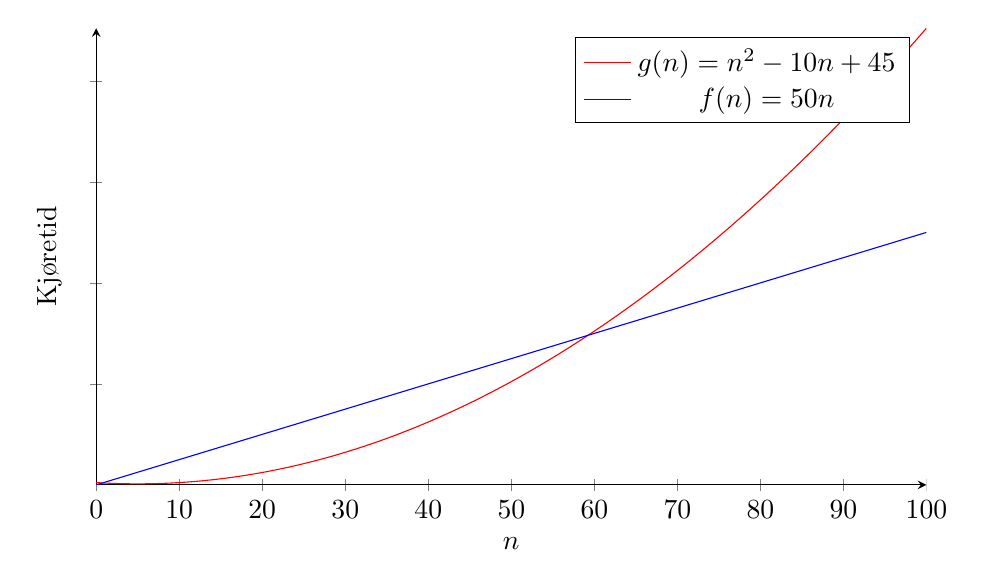
\begin{tikzpicture}
\begin{axis}[Big O]
\addplot [
    domain=0:100, 
    samples=100, 
    color=red,
]
{x^2 -10*x + 45};
\addlegendentry{$g(n) = n^2 -10n + 45$}
\addplot [
    domain=0:100, 
    samples=100, 
    color=blue,
    ]
    {50*x};
\addlegendentry{$f(n) = 50n$}

\end{axis}
\end{tikzpicture}
\end{frame}

\begin{frame}{}
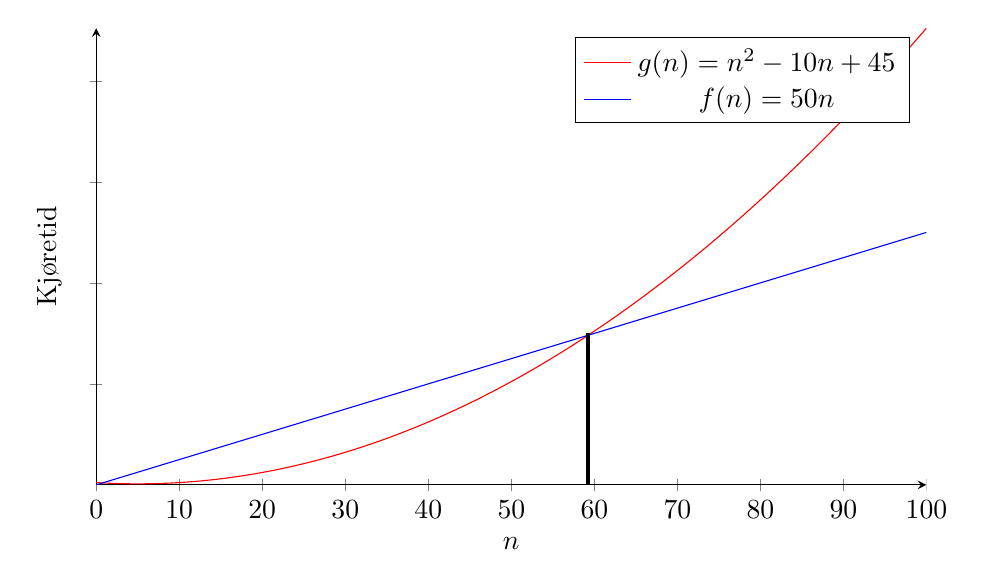
\begin{tikzpicture}
\begin{axis}[Big O]
\addplot [
    domain=0:100, 
    samples=100, 
    color=red,
]
{x^2 -10*x + 45};
\addlegendentry{$g(n) = n^2 -10n + 45$}
\addplot [
    domain=0:100, 
    samples=100, 
    color=blue,
    ]
    {50*x};
\addlegendentry{$f(n) = 50n$}
\addplot [smooth, very thick] coordinates {(59.24, 0) (59.24, 3000)};

\end{axis}
\end{tikzpicture}
\end{frame}

\begin{frame}{Kan se på det som intervaller}
    \begin{block}{}
    \vskip-2em
    Kan erstatte $n^2$ her med en hver funksjon $f(n)$. Merk forskjell mellom inklusiv og ekslusiv endepunkt.
			\begin{align*}
			\omega(n^2) &= (n^2, \infty)\\
			\Omega(n^2) &= [n^2, \infty)\\
			\Theta(n^2) &= [n^2, n^2]\\
			O(n^2) &= [1, n^2]\\
			o(n^2) &= [1, n^2)
			\end{align*}
			Da blir å legge sammen uttrykk det samme som å finne det intervallet som går fra største nedre grense til største øvre grense\footnote{\emph{Kun} når du er ute etter det mest presise, ellers blir det \emph{alle} intervaller som inkluderer den grensen vi beskrev.}
		\end{block}
\end{frame}	
\begin{frame}{Oppgave 2 H2017}
    \begin{block}{(5\%) a) Forenkle uttrykket $\Theta(n)+O(n^2) + \Omega(n^3)$}
    \begin{itemize}
        \item<2-> Vi får $[n, n] + [1, n^2] + [n^3, \infty) = [n^3, \infty] = \Omega(n^3)$
    \end{itemize}
    \end{block}
    \begin{block}{(5\%) b) Forenkle uttrykket $\Theta(n+\sqrt{n})+O(n^2+n) + \Omega(n\cdot(n+\lg{n}))$}
    %Lenke til LF: \url{https://algdat.idi.ntnu.no/arkiv/2017.des.tdt4120.losn.no.pdf}
    %Løsning:
    \begin{itemize}
        \item<3-> Vi forenkler: $\Theta(n+\sqrt{n}) \equiv \Theta(n)$, $O(n^2+n) \equiv O(n^2)$, $\Omega(n\cdot (n+\lg{n})) \equiv \Omega(n^2)$\\
        \item<4-> Vi får $[n, n] + [1, n^2] + [n^2, \infty) = [n^2, \infty] = \Omega(n^2)$
    \end{itemize}
    \end{block}
\end{frame}
\begin{frame}{Oppgave 10 Høst 2019}
    \begin{block}{(5\%) Hva er $O(n) + \Omega(n)+\Theta(n)+o(n) + \omega(n)$}
    \begin{itemize}
        \item<2-> $\Omega(n)$ kan bli vilkårlig stor, men $\omega(n)$ har et strengere minste-krav enn både $\Theta(n)$ og $\Omega(n)$, og dominerer derfor. Svar: $\omega(n)$
    \end{itemize}
    \end{block}
\end{frame}
\section{Rekurrenser}
\begin{frame}{Motivasjon}
    \begin{block}{Når funksjoner kaller på seg selv}
    \begin{pseudo}*
    \hd{Mystisk}(n) \\
    if $n > 1$ \\+
        \pr{Mystisk}(n-1)
\end{pseudo}
    
    \begin{itemize}
        \item<1-> Hvordan passer det inn i notasjonen vi nettopp lærte?
        \item<2-> Om en setter opp en funksjon, så får vi $f(n) = f(n-1) + 1$\\
        (Merk: vi må alltid sjekke if-en).
        \item<3-> Hva blir kjøretiden?
    \end{itemize}
    \end{block}
\end{frame}
\begin{frame}{Muligheter}
    \begin{block}{Når funksjoner kaller på seg selv}
Vi har forskjellige metoder
    \begin{itemize}
        \item Iterasjonsmetoden
        \item Substitusjon
        \item Rekursjonstre
        \item Masterteoremet\\
        \begin{itemize}
            \item Variabelskifte
        \end{itemize}
    \end{itemize}
    \end{block}
\end{frame} 
\begin{frame}{Iterasjonsmetoden}
    \begin{block}{Eksempeloppgave}
        La oss finne kjøretiden til funksjonen i forrige slide!
        \begin{pseudo}*
    \hd{Mystisk}(n) \\
    if $n > 1$ \\+
        \pr{Mystisk}(n-1)
\end{pseudo}
    
        Vi setter opp en rekurrensrelasjon: $T(n) = T(n-1) + 1$\\
        Hvor mange ganger må vi kalle \texttt{Mystisk} før vi når grunntilfellet $T(1) = 1$?
        \onslide<2->{Løsning: Vi reduserer $n$ med 1 hver gang, så vi må løse $n- k\cdot 1 = 1 \to k = n-1$.\footnote<2->{Hvorvidt vi utfører $n$ eller $n-1$ arbeid spiller sjelden en rolle} Så vi gjennomfører det konstante arbeidet $n$ ganger. Til sammen: $T(n) = n$, som er $\Theta(n)$}
    \end{block}
\end{frame} 
\begin{frame}{Substitusjon}
    \begin{block}{Kan vi ikke bare gjette oss frem?}
        Vi har fått et rekurrens $T(n) = 2T(n/2)+n$\\
        Jeg gjetter at løsningen ser ut som dette:\\
        $T(k)=k\lg{k}+k$, for $k<n$\\
        \begin{itemize}
            \item<2-> Hvordan kan vi sjekke dette?
            \item<3-> Induksjon!
        \end{itemize}
        
    \end{block}
\end{frame} 
\begin{frame}{Rekursjonstrær}
    \begin{block}{Iterasjonsmetoden med flere grener}
    \begin{itemize}
        \item Fin måte å visualisere arbeidet
        \item Kan være overveldene i starten
        \item<2-> Vi itererer gjennom hva algoritmen koster for hvert nivå i treet, og legger det sammen, altså får vi en sum ($\text{kostnad løvnivå} + \sum_{i=0}^{h-1}\text{pris for nivå $i$}$)
        \item<3-> Kjøretiden blir høyden til treet er hvor lang tid det tar å komme seg til grunntilfellet. Kjøretiden blir summen av kostnaden til hvert nivå
        \item<4-> Kan ofte bruke masterteoremet i stedet (men det bevises via rekurrensetrær)
        \item<5-> Eksempel: $T(n)=3T(n/4)+cn^2 = 3T(n/4) +\Theta(n^2)$. (s. 88 i boka)
    \end{itemize}
    \end{block}
\end{frame} 
{
\setbeamertemplate{navigation symbols}{}
\begin{frame}[plain]
    \makebox[\linewidth]{\includegraphics[height=\paperheight]{recursion-tree.png}}
\end{frame}
}
\begin{frame}{Rekursjonstrær}
    \begin{block}{Vi regner på det}
    \begin{itemize}
        \item For detaljer se boka
        \item For å telle noder på bunnen, benytter oss av $a^{\log{b}} = b^{\log{a}}$ (samme som vi benytter oss av i Masterteoremet)
        \item<2-> Antall noder ved høyde $h$ er $3^h$
        \item<3-> Teller antall noder på løvnivå: $3^{\log_4{n}} =n^{\log_4{3}}$, ved å anta konstant grunntilfelle får vi at kjøretiden blir $\Theta(n^{\log_4{3}})$
        \item<4-> Vi får følgende uttrykk: $T(n) =\sum_{i=0}^{\log_4{n}-1}\left(\frac{3}{16}\right)^i cn^2 + \Theta(n^{\log_4{3}} )$
        \item<5-> Regn ut selv!
        \item<6-> Hint: kan sammenligne med uendelig geometrisk rekke, hvordan påvirker det hvilken stor-O vi kan bruke?
    \end{itemize}
    \end{block}
\end{frame} 
\begin{frame}{Masterteoremet}
    \begin{block}{Master theorem}
    Let $a \geq 1$ and $b < 1$ be constants, let $f(n)$ be a function, and let $T(n)$ be defined on nonegative integers by the recurrence
    \[
    T(n) = aT(n/b)+f(n).
    \]
    where we interpret $n/b$ to mean either $\lfloor n/b\rfloor$ or $\lceil n/b \rceil$. Then $T(n)$ has the following asymptotic bounds:
    \begin{enumerate}
        \item If $f(n)=O(n^{\log_b{a-\epsilon}})$ for some constant $\epsilon > 0$, then $T(n)=\Theta(n^{\log_b{a}})$.
        \item If $f(n) = \Theta(n^{\log_b{a}})$, then $T(n) = \Theta(n^{\log_b{a}}\lg{n})$.
        \item If $f(n) = \Omega(n^{\log_b{a+\epsilon}})$ for some constant $\epsilon > 0$, and if $af(n/b) \leq cf(n)$ for some constant $c < 1$ and all sufficiently large $n$, then $T(n) = \Theta(f(n))$.
    \end{enumerate}
    \end{block}
\end{frame} 
\begin{frame}{Masterteoremet}
    \begin{block}{Hva gjør vi?}
    \begin{itemize}
        \item Vi sammenligner veksten mellom funksjon på rotnivå og kjøretiden til løvnivået i treet
        \begin{enumerate}
            \item Treet dominerer
            \item De er like
            \item Funksjonen dominerer, men OBS vi må sjekke at $f(n)$ \enquote{vokser normalt}, slik at treet ikke egentlig dominerer
        \end{enumerate}
        \item Vi finner ut av hva som dominerer, og dermed får vi en kjøretid
        \item Finnes mer generelle utgaver som takler flere rekurrenser, disse er \emph{ikke} pensum
        \item Flere tilfeller hvor vi ikke kan bruke det, står i boka.\\
        (Sjeldent det dukker opp i oppgaver)
    \end{itemize}
    \end{block}
\end{frame} 
\begin{frame}{Variabelskifte}
    \begin{block}{Bytt ut vanskelige uttrykk}
        \begin{itemize}
            \item Fremgangsmåte:
            \begin{enumerate}
                \item Sett opp ny rekurrens av en annen variabel, f.eks. $T(n) = T(2^k) = S(k)$
                \item Løs den, f.eks. med masterteoremet
                \item Bytt tilbake\footnote{Kan også benyttes dersom vi ikke har $T(n)$ på venstre side, da slipper vi å bytte tilbake} til $T(n)$, i vårt tilfelle blir det å sette $k=\log_2{n}$ siden $2^{\log_2{n}}=n$. Husk logaritme-base spiller sjelden en rolle
            \end{enumerate}
            \item Øving 3 har mye bra her
        \end{itemize}
    \end{block}
\end{frame}
\begin{frame}{Oppgave 3 K2015}
    \begin{block}{(5\%) Løs rekurrensen $T(n) = T(\sqrt{n})+\lg{n}$}
    \begin{enumerate}
        \item<2-> Hint: $m = \lg{n}$
        \item<3-> Hint: $S(m) = T(2^m)$
    \end{enumerate}
    %Vi får $[n, n] + [1, n^2] + [n^3, \infty) = [n^3, \infty] = \Omega(n^3)$
    \end{block}
\end{frame}
\begin{frame}{Å se kjøretid fra kode}
    \begin{block}{Må øves på}
    Gitt at vi har en funksjon FunctionN, som har kjøretid $\Theta(n)$, hva blir kjøretiden til disse?
    \begin{columns}
\begin{column}{0.5\textwidth}
        \begin{pseudo}*
    \hd{MystiskA}(n) \\
    if $n > 1$ \\+
        \pr{FunctionN}(n) \\
        $a = \pr{Mystisk}(n/2)$ \\
        $b = \pr{Mystisk}(n/2)$ \\
        $c = \pr{Mystisk}(n/2)$ \\
        return $a+b+c$
\end{pseudo}
Vi får rekurrens $T(n) = 3T(n/2) + \Theta(n)$, siden vi kaller funksjonen tre ganger.
\end{column}
\begin{column}{0.5\textwidth}  %%<--- here
    \begin{pseudo}*
    \hd{MystiskB}(n) \\
    if $n > 1$ \\+
        \pr{FunctionN}(n) \\
        return $3 \cdot \pr{Mystisk}(n/2)$
\end{pseudo}
Vi får rekurrense $T(n) = T(n/2) + \Theta(n)$, vi kaller bare funksjonen en gang!
\end{column}
\end{columns}
    \end{block}
\end{frame}

{
\setbeamertemplate{navigation symbols}{}
\begin{frame}[plain]
    \makebox[\linewidth]{\includegraphics[width=\paperwidth]{bg.png}}
\end{frame}
}

\section{Analyse}
\begin{frame}{Algoritmeanalyse}
    \begin{block}{Må øves på}
        Når vi regnet rekurrenser, så antok vi ingenting om hva $n$ var, så vi fant den generelle kjøretiden. Denne kjøretiden kan derimot variere veldig, basert på hvordan input ser ut. 
        \begin{itemize}
            \item Best-case, da antar vi noe om hvordan $n$ ser ut, utover størrelsen på data-en
            \item Worst-case, igjen vi antar noe om $n$
            \item Average-case, da kan vi anta en sannsynlighetsfordeling for input, f.eks. vi antar at vi vanligvis får nesten-sorterte lister. Da må vi vite mer om nøyaktig hva algoritmen brukes til
            \item Amortisert analyse: Da ser vi på gjennomsnitt av kjøretiden over flere kall av algoritmen, men vi antar ingenting om $n$. Eksempel
        \end{itemize}
    \end{block}
\end{frame}

\begin{frame}{Amortisert Analyse}
    \begin{block}{Innsetting i \texttt{std::vector}, eller Java sin \texttt{ArrayList}}
\begin{pseudo}*
\hd{Table-Insert}(T,x)\\
if $T.size \== 0$\\+
    \tn{allocate $T.table$ with 1 slot}\\
    $T.size \== 1$\\-
if $T.num \== T.size$\\+
    \tn{allocate \id{new-table} with $2\cdot T.size$ slots}\\
    \tn{insert all items in $T.table$ into \id{new-table}}\\
    \tn{free $T.table$}\\
    $T.table = \id{new-table}$\\
    $T.size = 2\cdot T.size$\\-
\tn{insert $x$ into $T.table$}\\
$T.num = T.num + 1$
\end{pseudo}
    \end{block}
\end{frame}

\section{Sortering}
\begin{frame}{Egenskaper}
    \begin{block}{Forskjellige algoritmer, ulike egenskaper}
        \begin{itemize}
            \item Sammenligningsbasert (\enquote{generell}) eller ikke (\enquote{spesialisert})
            \item Best / Average / Worst case kjøretid
            \item Minnebruk - in-place
            \item Stabil: dersom du sorterer en liste med like elementer, havner de på samme plass?
            \item Finnes mange flere, som ikke er relevant for dette faget:
            \begin{itemize}
                \item Parallelliserbar
                \item Online --- betyr at du løser problemet mens du kun har fått deler av det, tenk få ett og ett tall vs. hele listen.
            \end{itemize}
        \end{itemize}
    \end{block}
\end{frame}

\begin{frame}{Diggresjon}
    \begin{block}{Hvorfor lærer vi masse sortering}
        \begin{itemize}
            \item I praksis bruker vi oftest bare en innebygd \texttt{.sort()}-metode
            \item Forskjellige måter å bryte ned et problem på
            \item Disse måtene har forskjellige egenskaper
            \item Dere skal lære mye mer enn det jeg får fortalt i dag, spesielt å konstruere \emph{nye} algoritmer, det må en øve på selv! Ikke se på LF først!
            \item Sortering er en naturlig del av mange andre problemer
        \end{itemize}
    \end{block}
\end{frame}

\begin{frame}{Læringsmål}
    \begin{block}{Minner om at følgende gjelder for \emph{alle} algoritmer i pensum}
        \begin{itemize}
            \item Kjenne den formelle definisjonen av det generelle problemet den løser
            \item<2-> Kjenne til eventuelle tilleggskrav den stiller for å være korrekt
            \item<3-> Vite hvordan den oppfører seg; kunne utføre algoritmen, trinn for trinn
            \item<4-> \textbf{!} Forstå korrekthetsbeviset; hvordan og hvorfor virker algoritmen egentlig?
            \item<5-> Kjenne til eventuelle styrker eller svakheter, sammenlignet med andre
            \item<6-> Kjenne kjøretidene under ulike omstendigheter, og forstå utregningen
        \end{itemize}
        \onslide<7->{\textbf{Altså:} Det finnes cheat-sheets, men en må likevel forstå algoritmen til den grad at du kan skrive den i pseudo-kode-form!}
    \end{block}
\end{frame}

\begin{frame}{Insertion sort}
    \begin{block}{}
    \begin{columns}
\begin{column}{0.5\textwidth}
Slik vi vanligvis sorterer en kortstokk.
\begin{table}[b]
    \centering
    \begin{tabular}{|c|c|}
    \hline
    Sammenligning & Ja\\
    \hline
    Best-case & $\Theta(n)$\\
    \hline
    Average-case & $\Theta(n^2)$\\
    \hline
    Worst-case & $\Theta(n^2)$\\
    \hline
    Minne & $O(1)$\\
    \hline
    In-place & Ja\\
    \hline
    Stabil & Ja\\
    \hline
\end{tabular}
\end{table}

\end{column}
\begin{column}{0.5\textwidth}
\animategraphics[loop,controls,width=\textwidth]{16}{images/gifs/insertion-sort/insertion-sort-}{0}{210}
\end{column}
\end{columns}
    \end{block}
\end{frame} 
\begin{frame}{Merge sort}
    \begin{block}{}
    \begin{columns}
\begin{column}{0.5\textwidth}
En liste med ett element er sortert, vi kan så flette disse sammen raskt.
\begin{table}[b]
    \centering
    \begin{tabular}{|c|c|}
        \hline
        Sammenligning & Ja\\
        \hline
        Best-case & $\Theta(n\lg{n})$\\
        \hline
        Average-case & $\Theta(n\lg{n})$\\
        \hline
        Worst-case & $\Theta(n\lg{n})$\\
        \hline
        Minne & $O(n)$\\
        \hline
        In-place & Nei\\
        \hline
        Stabil & Ja\\
        \hline
    \end{tabular}
\end{table}
\end{column}
\begin{column}{0.5\textwidth}
\animategraphics[loop,controls,width=\textwidth]{16}{images/gifs/insertion-sort/insertion-sort-}{0}{210}
\end{column}
\end{columns}
    \end{block}
\end{frame} 
\begin{frame}{Quicksort}
    \begin{block}{}
    \begin{columns}
\begin{column}{0.5\textwidth}
\begin{itemize}
    \item Velg et pivot-element, splitt tabellen i to, en halvdel er større, andre er mindre.
    \item Splitt og hersk.
    \item Problem: allerede sortert liste, og du velger største element. Løsning: tilfeldig pivot!
\end{itemize}
(\enquote{Pivot} betyr \enquote{dreie}, så elementet blir der vi bytter mellom mindre enn og større enn)
\end{column}
\begin{column}{0.5\textwidth}
\animategraphics[loop,controls,width=\textwidth]{16}{images/gifs/insertion-sort/insertion-sort-}{0}{210}
\end{column}
\end{columns}
    \end{block}
\end{frame} 
\begin{frame}{Quicksort}
    \begin{block}{}
    \begin{columns}
\begin{column}{0.5\textwidth}
\begin{table}[b]
    \centering
    \begin{tabular}{|c|c|}
        \hline
        Sammenligning & Ja\\
        \hline
        Best-case & $\Theta(n\lg{n})$\\
        \hline
        Average-case & $\Theta(n\lg{n})$\\
        \hline
        Worst-case & $\Theta(n^2)$\\
        \hline
        Minne & $O(\lg{n})$\\
        \hline
        In-place & Ja\\
        \hline
        Stabil & Nei\\
        \hline
    \end{tabular}
\end{table}
\end{column}
\begin{column}{0.5\textwidth}
\animategraphics[loop,controls,width=\textwidth]{3}{images/gifs/quicksort/quicksort-}{0}{69}
\end{column}
\end{columns}
    \end{block}
\end{frame} 

\begin{frame}{Heapsort}
    \begin{block}{}
    \begin{columns}
\begin{column}{0.5\textwidth}
Lag en max-heap -- hent største element -- reduser størrelsen på heapen og gjør den til en heap igjen -- repeat
\begin{table}[b]
    \centering
    \begin{tabular}{|c|c|}
        \hline
        Sammenligning & Ja\\
        \hline
        Best-case & $\Theta(n\lg{n})$\\
        \hline
        Average-case & $\Theta(n\lg{n})$\\
        \hline
        Worst-case & $\Theta(n\lg{n})$\\
        \hline
        Minne & $O(1)$\\
        \hline
        In-place & Ja\\
        \hline
        Stabil & Nei\\
        \hline
    \end{tabular}
\end{table}
\end{column}
\begin{column}{0.5\textwidth}
\animategraphics[loop,controls,width=\textwidth]{16}{images/gifs/insertion-sort/insertion-sort-}{0}{210}
\end{column}
\end{columns}
    \end{block}
\end{frame} 
\begin{frame}{Sorteringsgrense}
    \begin{block}{Sorteringsgrensen}
        Any comparison sort algorithm requires $\Omega(n\lg{n})$ comparisons in the worst case.
    \end{block}
    \begin{block}{Konsekvenser}
    Det er umulig å sortere raskere, uten å anta egenskaper ved problemet. Bevis i boka.
    \end{block}
\end{frame} 
\input{slides/sorting/08-counting}
\input{slides/sorting/09-radix}
\begin{frame}{Bucket sort}
    \begin{block}{}
    \begin{columns}
\begin{column}{0.5\textwidth}
Uniformt fordel tallene i bøtter, sorter så i hver bøtte og kombiner. NB: krever uniform sannsynlighetsfordeling! \\
*: avhenger av sub-rutine
\begin{table}[b]
    \centering
    \begin{tabular}{|c|c|}
        \hline
        Sammenligning & Nei*\\
        \hline
        Best-case & $\Theta(n)$\\
        \hline
        Average-case & $\Theta(n)$\\
        \hline
        Worst-case & $\Theta(n^2)$\\
        \hline
        Minne & $O(n)$\\
        \hline
        In-place & Nei\\
        \hline
        Stabil & Ja*\\
        \hline
    \end{tabular}
    \end{table}
\end{column}
\begin{column}{0.5\textwidth}
\includegraphics[width=\textwidth]{images/bucketsort.png}
\end{column}
\end{columns}
    \end{block}
\end{frame} 
\begin{frame}{Oppgave 2 Høst 2011}
    \begin{block}{(7\%) Oppgave c}
        En venn av deg påstår han har utviklet en generell prioritetskø der operasjonene for å legge til et element, å finne maksimum og å ta ut maksimum alle har kjøretid $O(1)$ i verste tilfelle. Forklar hvorfor dette ikke kan stemme.
        \begin{itemize}
            \item<2-> Løsning: Vi kan brukke dette til å sortere i $O(n)$ tid generelt, det bryter med fartsgrensen vår.
        \end{itemize}
    \end{block}
\end{frame} 

\begin{frame}{Oppgave 1 Høst 2010}
    \begin{block}{(5\%) Oppgave g}
        \textsc{Heapsort} er optimal, men \textsc{Radix-Sort} har bedre asymptotisk kjøretid. Forklar svært kort hvordan dette henger sammen.
        \begin{itemize}
            \item<2-> Løsning: \textsc{Heapsort} løser det generelle sorteringsproblemet (sammenligningsbasert). \textsc{Radix-Sort} gjør antagelser.
        \end{itemize}
    \end{block}
\end{frame} 

\begin{frame}{Oppgave 3 Høst 2014}
    \begin{block}{(5\%) Oppgave a}
        Du ønsker å sortere sekvensen $A = (a_1,a_2,\ldots,a_n)$. Det er velkjent at for sammenligningsbasert sortering er $\Omega(n\log{n})$ den beste kjøretiden vi kan få, i forventet (\textit{average-case}) og verste tilfelle.\\
        Anta at elementene er reelle tall, distribuert etter en gitt sannsynlighetsfordeling, som kan beregnes i konstant tid for ethvert element. Hva er den beste forventede kjøretiden vi kan få, og hvordan kan du oppnå den? Forklart kort.
        \begin{itemize}
            \item<2-> Løsning: Spesialtilfelle av Bucket-sort
        \end{itemize}
    \end{block}
\end{frame} 


\end{document}